%!TEX root = report.tex

The following discussion relies primarily on the book by Cheng \cite{cheng} and the book by Carroll \cite{carroll} although some other references have been used, and they are referenced in the text.

\section{The Equivalence Principle}

The fundamental idea which caused Einstein to suggest that relativistic physics occurs on a 4 dimensional differentiable manifold is the equivalence principle. The equivalence principle states that physical laws in a freely falling frame of reference must be the same as those in an inertial frame without gravity. Thus, any point of spacetime must locally look like the flat spacetime of special relativity \cite{cheng, carroll}. 

The principle of equivalence had already existed in a simpler form before Einstein, as a statement that the inertial mass of an object and the gravitational mass were equivalent. This statement had already received experimental verification in various forms, first by Galileo (the story of dropping two balls of different mass from the Leaning Tower of Pisa seems to be apocryphal) and Newton, and then later in a more sophisticated form of the E{\" o}tv{\" o}s experiment \cite{cheng}. 

Einstein extended this principle from just motion in inertial frames to any frame of reference using any coordinate system. In order to capture this coordinate free description of physics Einstein turned to differential geometry and tensors. This mathematical formalism was chosen due to a differentiable manifold locally looking like flat space, but globally potentially having curvature. This condition replicates that of the equivalence principle: in small regions of space we can easily transform the metric to look like the flat space metric, and thus return to special relativity, but globally this is not possible \cite{cheng, carroll, szekeres}. 

\section{Manifolds, Vectors and Tensors}

The fundamental object in differential geometry is a differentiable manifold \(M\). A differentiable manifold is an \(n\)-dimensional space which locally looks like the equivalent flat \(\mathbb{R}^n\) space but may have global curvature, unlike flat space. In the case of relativity we use a 4-dimensional manifold which we call spacetime. Points on this manifold are called events and are a combination of both the time coordinate and the space coordinates. We then have local coordinates \(x^{\mu}\) on this manifold. In the relativistic case greek indices will run from 0 to 3, with the 0 index being the time coordinate and 1 to 3 being spatial. 

At all points \(p\) on the manifold we have the tangent space \(T_p (M)\). The tangent space is the vector space of all possible tangent vectors at a point \(p\) on the manifold. The basis vectors of the tangent space can be taken to be the partial derivative operators at that point and thus are tangential to the manifold at that point. That is

\begin{equation} \label{coordinate-basis}
	\hat{e}_{\mu} = \partial_{\mu} = \frac{\partial}{\partial x^{\mu}} .
\end{equation}

This is the basis we will use while studying General Relativity and we call this the coordinate basis. As an example in 2D we could visualise this as a plane intersecting a manifold at a point \footnote{Edited from original file at \url{http://commons.wikimedia.org/wiki/File:Tangentialvektor.png}}.

%\newpage

%%LaTeX with PSTricks extensions
%%Creator: inkscape 0.48.3.1
%%Please note this file requires PSTricks extensions
\psset{xunit=.5pt,yunit=.5pt,runit=.5pt}
\begin{pspicture}(640,440)
{
\newrgbcolor{curcolor}{1 1 1}
\pscustom[linestyle=none,fillstyle=solid,fillcolor=curcolor]
{
\newpath
\moveto(0,440)
\lineto(640,440)
\lineto(640,0)
\lineto(0,0)
\closepath
}
}
{
\newrgbcolor{curcolor}{0.2 0.2 0.2}
\pscustom[linestyle=none,fillstyle=solid,fillcolor=curcolor]
{
\newpath
\moveto(120,20)
\curveto(71.859661,199.85966)(39.456158,271.49119)(20,260)
\curveto(216.59639,387.052655)(434.10531,349.842146)(600,140)
\curveto(472.87707,208.36847)(325.89469,163.71932)(120,20)
\closepath
}
}
{
\newrgbcolor{curcolor}{0.88235295 0.88235295 0.88235295}
\pscustom[linewidth=1,linecolor=curcolor,strokeopacity=0.2590909]
{
\newpath
\moveto(102.6295059,133.3665552)
\lineto(12.6295059,323.3665552)
\lineto(322.6295059,363.3665552)
\lineto(602.6295059,263.3665552)
\lineto(102.6295059,133.3665552)
}
}
{
\newrgbcolor{curcolor}{1 1 1}
\pscustom[linestyle=none,fillstyle=solid,fillcolor=curcolor]
{
\newpath
\moveto(270,300)
\curveto(270,296.6862915)(263.28427125,294)(255,294)
\curveto(246.71572875,294)(240,296.6862915)(240,300)
\curveto(240,303.3137085)(246.71572875,306)(255,306)
\curveto(263.28427125,306)(270,303.3137085)(270,300)
\closepath
}
}
{
\newrgbcolor{curcolor}{0 0 0}
\pscustom[linestyle=none,fillstyle=solid,fillcolor=curcolor]
{
\newpath
\moveto(346.384,422.344)
\lineto(320.848,422.344)
\lineto(318.832,414.952)
\lineto(319.696,414.76)
\curveto(322.23999746,419.94399482)(323.77600734,420.7599999)(331.12,420.664)
\lineto(324.208,395.32)
\curveto(323.44000077,392.77600254)(322.28799683,392.00799976)(319.12,391.768)
\lineto(319.12,391)
\lineto(333.04,391)
\lineto(333.04,391.768)
\curveto(332.22400082,391.81599995)(331.50399971,391.912)(331.216,391.912)
\curveto(329.29600192,392.05599986)(328.72,392.48800144)(328.72,393.928)
\curveto(328.72,394.55199938)(328.86400043,395.12800163)(329.296,396.76)
\lineto(335.968,420.664)
\lineto(338.608,420.664)
\curveto(342.06399654,420.664)(343.6,419.46399731)(343.6,416.776)
\curveto(343.6,416.15200062)(343.5519999,415.43199918)(343.456,414.616)
\lineto(344.272,414.52)
\lineto(346.384,422.344)
}
}
{
\newrgbcolor{curcolor}{0 0 0}
\pscustom[linestyle=none,fillstyle=solid,fillcolor=curcolor]
{
\newpath
\moveto(344.46597461,394.00497716)
\lineto(345.18358472,394.00497716)
\curveto(345.18358472,394.00497716)(345.24598563,394.00497719)(345.27718604,394.0361776)
\curveto(345.68279134,394.22338005)(346.49400317,393.63057142)(346.49400317,393.16256529)
\curveto(346.49400317,392.88176162)(345.37078626,388.45129482)(344.27877197,384.33284093)
\curveto(343.43636095,381.2128001)(342.68754934,378.24875433)(342.46914648,377.34394249)
\curveto(342.12594199,375.90872371)(341.7203346,375.53431697)(340.37871704,375.50311656)
\lineto(340.37871704,375.00390953)
\lineto(346.77480713,375.00390953)
\lineto(346.77480713,375.47191612)
\curveto(345.30838794,375.47191612)(344.777979,375.75272073)(344.777979,376.40792931)
\curveto(344.777979,376.84473502)(345.3083871,379.27837204)(345.93239526,381.58720226)
\curveto(346.71240547,381.18159695)(347.27401488,381.05679478)(347.99162427,381.05679478)
\curveto(352.54688387,381.05679478)(357.3517561,386.29847357)(357.3517561,391.25933849)
\curveto(357.3517561,393.69297033)(355.97893455,395.15939342)(353.76370557,395.15939342)
\curveto(351.73567903,395.15939342)(350.2380541,394.16097683)(348.42843042,391.63374376)
\lineto(349.33324316,394.7537877)
\lineto(349.42684448,395.03459166)
\curveto(349.42684448,395.03459166)(349.39564401,395.06579216)(349.3644436,395.12819298)
\lineto(349.30204272,395.15939342)
\curveto(349.30204272,395.19059383)(349.27084229,395.19059386)(349.27084229,395.19059386)
\lineto(349.20844141,395.15939342)
\lineto(344.40357373,394.47298375)
\lineto(344.46597461,394.00497716)
\moveto(352.60928931,393.81777452)
\curveto(353.95090686,393.7553737)(354.54371655,392.94416041)(354.54371655,391.13453673)
\curveto(354.54371655,389.07530978)(353.63890247,386.392068)(352.29728491,384.45764268)
\curveto(350.98686777,382.6168186)(349.48924374,381.64960313)(347.86682251,381.64960313)
\curveto(346.99321108,381.64960313)(346.36920142,382.11761041)(346.36920142,382.80401939)
\curveto(346.36920142,383.86483327)(347.49241814,387.95209421)(348.39722998,390.26092442)
\curveto(349.239641,392.38255218)(351.04926889,393.91137575)(352.60928931,393.81777452)
}
}
{
\newrgbcolor{curcolor}{0 0 0}
\pscustom[linestyle=none,fillstyle=solid,fillcolor=curcolor]
{
\newpath
\moveto(400.22296973,421.63400002)
\lineto(392.20696973,421.63400002)
\lineto(376.07896973,397.97000002)
\lineto(373.43896973,421.63400002)
\lineto(364.75096973,421.63400002)
\lineto(364.75096973,420.86600002)
\curveto(367.15096733,420.72200017)(368.30296973,420.19399892)(368.30296973,419.09000002)
\curveto(368.30296973,418.70600041)(368.11096944,417.98599916)(367.82296973,417.12200002)
\curveto(367.72696982,416.93000021)(367.58296953,416.4019993)(367.39096973,415.68200002)
\curveto(367.34296977,415.53800017)(367.29496968,415.34599983)(367.24696973,415.15400002)
\lineto(362.15896973,397.29800002)
\curveto(360.67097121,392.30600501)(359.95096723,391.34599973)(357.45496973,391.05800002)
\lineto(357.45496973,390.29000002)
\lineto(366.95896973,390.29000002)
\lineto(366.95896973,391.05800002)
\curveto(364.51097217,391.24999983)(363.55096973,391.82600137)(363.55096973,393.17000002)
\curveto(363.55096973,393.64999954)(363.74296997,394.89800084)(363.98296973,395.71400002)
\lineto(369.64696973,416.49800002)
\lineto(372.57496973,390.29000002)
\lineto(373.39096973,390.29000002)
\lineto(391.48696973,417.21800002)
\lineto(385.29496973,394.65800002)
\curveto(384.52697049,392.11400257)(383.56696661,391.39399969)(380.44696973,391.05800002)
\lineto(380.44696973,390.29000002)
\lineto(393.55096973,390.29000002)
\lineto(393.55096973,391.05800002)
\curveto(390.28697299,391.34599973)(389.85496973,391.63400151)(389.85496973,393.12200002)
\curveto(389.85496973,393.93799921)(389.95097016,394.56200151)(390.38296973,396.05000002)
\lineto(396.28696973,417.31400002)
\curveto(397.15096886,420.19399714)(397.39097256,420.43400045)(400.22296973,420.86600002)
\lineto(400.22296973,421.63400002)
}
}
{
\newrgbcolor{curcolor}{0 0 0}
\pscustom[linestyle=none,fillstyle=solid,fillcolor=curcolor]
{
\newpath
\moveto(460.904,153.344)
\lineto(452.888,153.344)
\lineto(436.76,129.68)
\lineto(434.12,153.344)
\lineto(425.432,153.344)
\lineto(425.432,152.576)
\curveto(427.8319976,152.43200014)(428.984,151.9039989)(428.984,150.8)
\curveto(428.984,150.41600038)(428.79199971,149.69599914)(428.504,148.832)
\curveto(428.4080001,148.64000019)(428.26399981,148.11199928)(428.072,147.392)
\curveto(428.02400005,147.24800014)(427.97599995,147.05599981)(427.928,146.864)
\lineto(422.84,129.008)
\curveto(421.35200149,124.01600499)(420.6319975,123.05599971)(418.136,122.768)
\lineto(418.136,122)
\lineto(427.64,122)
\lineto(427.64,122.768)
\curveto(425.19200245,122.95999981)(424.232,123.53600134)(424.232,124.88)
\curveto(424.232,125.35999952)(424.42400024,126.60800082)(424.664,127.424)
\lineto(430.328,148.208)
\lineto(433.256,122)
\lineto(434.072,122)
\lineto(452.168,148.928)
\lineto(445.976,126.368)
\curveto(445.20800077,123.82400254)(444.24799688,123.10399966)(441.128,122.768)
\lineto(441.128,122)
\lineto(454.232,122)
\lineto(454.232,122.768)
\curveto(450.96800326,123.05599971)(450.536,123.34400149)(450.536,124.832)
\curveto(450.536,125.64799918)(450.63200043,126.27200149)(451.064,127.76)
\lineto(456.968,149.024)
\curveto(457.83199914,151.90399712)(458.07200283,152.14400043)(460.904,152.576)
\lineto(460.904,153.344)
}
}
{
\newrgbcolor{curcolor}{0 0 0}
\pscustom[linestyle=none,fillstyle=solid,fillcolor=curcolor]
{
\newpath
\moveto(293.52553786,289.81323846)
\curveto(293.52551801,291.72728557)(293.10885176,293.19212785)(292.27553786,294.20776971)
\curveto(291.44218676,295.22337582)(290.24427129,295.73118781)(288.68178786,295.73120721)
\curveto(287.61406559,295.73118781)(286.5919312,295.45775059)(285.61538161,294.91089471)
\curveto(284.65182897,294.36400168)(283.79245483,293.56973164)(283.03725661,292.52808221)
\curveto(282.29506049,291.49942121)(281.70261317,290.25593287)(281.25991286,288.79761346)
\curveto(280.81719739,287.33926912)(280.59584344,285.89395807)(280.59585036,284.46167596)
\curveto(280.59584344,282.63875299)(281.01250969,281.23250439)(281.84585036,280.24292596)
\curveto(282.67917469,279.26636053)(283.86406934,278.77807977)(285.40053786,278.77808221)
\curveto(286.53333751,278.77807977)(287.58151354,279.04500658)(288.54506911,279.57886346)
\curveto(289.52161577,280.11271385)(290.35494827,280.88745266)(291.04506911,281.90308221)
\curveto(291.7872385,282.97078391)(292.38619624,284.22729307)(292.84194411,285.67261346)
\curveto(293.29765366,287.11791518)(293.52551801,288.49812213)(293.52553786,289.81323846)
\moveto(282.39272536,294.89136346)
\curveto(283.35625735,296.15436447)(284.48906872,297.11139477)(285.79116286,297.76245721)
\curveto(287.1062536,298.4134768)(288.56458547,298.7389973)(290.16616286,298.73901971)
\curveto(292.40572747,298.7389973)(294.14400698,298.00332096)(295.38100661,296.53198846)
\curveto(296.61796284,295.07363639)(297.2364518,293.02285719)(297.23647536,290.37964471)
\curveto(297.2364518,288.21817449)(296.8523376,286.15437447)(296.08413161,284.18823846)
\curveto(295.31588081,282.23510756)(294.20911108,280.48380723)(292.76381911,278.93433221)
\curveto(291.80025932,277.9056848)(290.71302083,277.11792518)(289.50210036,276.57105096)
\curveto(288.29114825,276.03719709)(287.01510786,275.77027027)(285.67397536,275.77026971)
\curveto(284.12448575,275.77027027)(282.82240372,276.08928037)(281.76772536,276.72730096)
\curveto(280.71303083,277.37834158)(279.9252712,278.34188229)(279.40444411,279.61792596)
\lineto(277.15835036,268.01636346)
\lineto(273.56460036,268.01636346)
\lineto(279.44350661,298.21167596)
\lineto(283.03725661,298.21167596)
\lineto(282.39272536,294.89136346)
}
}
{
\newrgbcolor{curcolor}{0 0 0}
\pscustom[linestyle=none,fillstyle=solid,fillcolor=curcolor]
{
\newpath
\moveto(70.45886265,263.23676631)
\curveto(68.62291845,263.23676687)(67.10599288,263.79015174)(65.9080814,264.89692256)
\curveto(64.488808,266.21202431)(63.77917329,268.0609808)(63.77917515,270.44379756)
\curveto(63.77917329,272.91774678)(64.40417267,275.11826541)(65.65417515,277.04536006)
\curveto(66.94323263,279.0245115)(68.74661624,280.01409385)(71.0643314,280.01411006)
\curveto(72.58775824,280.01409385)(73.94843396,279.5388339)(75.14636265,278.58832881)
\curveto(75.84947372,278.02841875)(76.44192105,277.27972158)(76.9237064,276.34223506)
\curveto(77.09296206,277.39690896)(77.1775974,278.52320992)(77.17761265,279.72114131)
\curveto(77.1775974,281.47893613)(76.96926427,282.86565349)(76.55261265,283.88129756)
\curveto(75.62811978,286.13387939)(73.94192355,287.26018035)(71.4940189,287.26020381)
\curveto(70.56953109,287.26018035)(69.39114685,286.9737223)(67.95886265,286.40082881)
\lineto(67.95886265,289.68207881)
\curveto(69.46927177,290.08569836)(70.90156201,290.28752107)(72.25573765,290.28754756)
\curveto(75.74530716,290.28752107)(78.23228384,288.68596017)(79.71667515,285.48286006)
\curveto(80.40676083,283.97242322)(80.75181257,282.09091469)(80.7518314,279.83832881)
\curveto(80.75181257,278.36696008)(80.58905232,276.77842)(80.26355015,275.07270381)
\curveto(79.44322013,270.80186348)(77.97186744,267.65082496)(75.84948765,265.61957881)
\curveto(74.18280872,264.03103691)(72.38593552,263.23676687)(70.45886265,263.23676631)
\moveto(67.1190189,269.85786006)
\curveto(67.1190137,268.55577197)(67.40547175,267.55316881)(67.9783939,266.85004756)
\curveto(68.5903664,266.10785775)(69.36510521,265.73676437)(70.30261265,265.73676631)
\curveto(71.13593677,265.73676437)(71.88463394,266.02973283)(72.5487064,266.61567256)
\curveto(73.48619484,267.4229606)(74.29999611,268.48415746)(74.99011265,269.79926631)
\curveto(75.56301568,270.8799884)(75.99270275,271.99977894)(76.27917515,273.15864131)
\curveto(75.12030779,275.95810832)(73.53827812,277.3578465)(71.5330814,277.35786006)
\curveto(69.81432351,277.3578465)(68.57734558,276.22503514)(67.8221439,273.95942256)
\curveto(67.35338847,272.55316381)(67.1190137,271.18597767)(67.1190189,269.85786006)
}
}
{
\newrgbcolor{curcolor}{0 0 0}
\pscustom[linestyle=none,fillstyle=solid,fillcolor=curcolor]
{
\newpath
\moveto(85.85148619,257.96140608)
\lineto(90.04099833,257.96140608)
\lineto(90.04099833,272.42157069)
\lineto(85.48331695,271.50749531)
\lineto(85.48331695,273.84346571)
\lineto(90.01560734,274.75754109)
\lineto(92.58009659,274.75754109)
\lineto(92.58009659,257.96140608)
\lineto(96.76960872,257.96140608)
\lineto(96.76960872,255.80317256)
\lineto(85.85148619,255.80317256)
\lineto(85.85148619,257.96140608)
}
}
{
\newrgbcolor{curcolor}{0 0 0}
\pscustom[linestyle=none,fillstyle=solid,fillcolor=curcolor]
{
\newpath
\moveto(224.49064636,351.74320984)
\curveto(222.65470216,351.74321041)(221.1377766,352.29659527)(219.93986511,353.40336609)
\curveto(218.52059171,354.71846785)(217.81095701,356.56742433)(217.81095886,358.95024109)
\curveto(217.81095701,361.42419031)(218.43595638,363.62470894)(219.68595886,365.55180359)
\curveto(220.97501634,367.53095503)(222.77839996,368.52053738)(225.09611511,368.52055359)
\curveto(226.61954195,368.52053738)(227.98021767,368.04527744)(229.17814636,367.09477234)
\curveto(229.88125744,366.53486228)(230.47370476,365.78616511)(230.95549011,364.84867859)
\curveto(231.12474578,365.9033525)(231.20938111,367.02965345)(231.20939636,368.22758484)
\curveto(231.20938111,369.98537966)(231.00104798,371.37209703)(230.58439636,372.38774109)
\curveto(229.65990349,374.64032292)(227.97370726,375.76662388)(225.52580261,375.76664734)
\curveto(224.6013148,375.76662388)(223.42293056,375.48016583)(221.99064636,374.90727234)
\lineto(221.99064636,378.18852234)
\curveto(223.50105548,378.59214189)(224.93334572,378.7939646)(226.28752136,378.79399109)
\curveto(229.77709087,378.7939646)(232.26406755,377.19240371)(233.74845886,373.98930359)
\curveto(234.43854455,372.47886675)(234.78359628,370.59735822)(234.78361511,368.34477234)
\curveto(234.78359628,366.87340361)(234.62083603,365.28486353)(234.29533386,363.57914734)
\curveto(233.47500384,359.30830701)(232.00365115,356.15726849)(229.88127136,354.12602234)
\curveto(228.21459244,352.53748044)(226.41771923,351.74321041)(224.49064636,351.74320984)
\moveto(221.15080261,358.36430359)
\curveto(221.15079742,357.0622155)(221.43725546,356.05961234)(222.01017761,355.35649109)
\curveto(222.62215011,354.61430128)(223.39688892,354.24320791)(224.33439636,354.24320984)
\curveto(225.16772048,354.24320791)(225.91641765,354.53617636)(226.58049011,355.12211609)
\curveto(227.51797855,355.92940414)(228.33177982,356.99060099)(229.02189636,358.30570984)
\curveto(229.59479939,359.38643193)(230.02448646,360.50622248)(230.31095886,361.66508484)
\curveto(229.1520915,364.46455185)(227.57006183,365.86429003)(225.56486511,365.86430359)
\curveto(223.84610722,365.86429003)(222.60912929,364.73147867)(221.85392761,362.46586609)
\curveto(221.38517218,361.05960734)(221.15079742,359.69242121)(221.15080261,358.36430359)
}
}
{
\newrgbcolor{curcolor}{0 0 0}
\pscustom[linestyle=none,fillstyle=solid,fillcolor=curcolor]
{
\newpath
\moveto(241.6479432,346.46784961)
\lineto(250.59826458,346.46784961)
\lineto(250.59826458,344.30961609)
\lineto(238.56293881,344.30961609)
\lineto(238.56293881,346.46784961)
\curveto(239.53625693,347.47502209)(240.86081854,348.82497465)(242.53662759,350.51771134)
\curveto(244.22088854,352.21889927)(245.27884509,353.31494226)(245.71050042,353.80584359)
\curveto(246.53146565,354.72837221)(247.10276219,355.50702823)(247.42439175,356.14181399)
\curveto(247.75446342,356.78503974)(247.91950465,357.41558185)(247.91951591,358.0334422)
\curveto(247.91950465,359.04060311)(247.56403125,359.8615774)(246.85309464,360.49636751)
\curveto(246.15060129,361.13112526)(245.23229501,361.44851222)(244.09817302,361.44852936)
\curveto(243.2941186,361.44851222)(242.44352154,361.30886196)(241.54637927,361.02957815)
\curveto(240.65769088,360.7502609)(239.70552998,360.32707828)(238.68989372,359.76002902)
\lineto(238.68989372,362.34990925)
\curveto(239.72245729,362.76461017)(240.68731366,363.07776531)(241.58446574,363.2893756)
\curveto(242.48160797,363.50094793)(243.30258226,363.60674359)(244.04739106,363.60676289)
\curveto(246.01095103,363.60674359)(247.57672672,363.11585175)(248.74472284,362.13408589)
\curveto(249.91269479,361.15228439)(250.49668681,359.84041827)(250.49670064,358.19848359)
\curveto(250.49668681,357.41981368)(250.34857289,356.67924409)(250.05235845,355.97677261)
\curveto(249.76458087,355.28274144)(249.2356026,354.46176716)(248.46542203,353.51384729)
\curveto(248.25381892,353.26839217)(247.58095855,352.55744536)(246.44683892,351.38100475)
\curveto(245.3126997,350.21301365)(243.7130694,348.5752969)(241.6479432,346.46784961)
}
}
\end{pspicture}

% need some caption here
%\begin{center}
%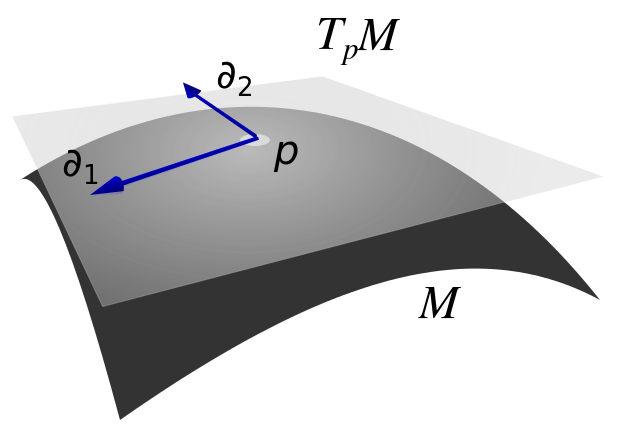
\includegraphics[scale=0.3]{Tangentialvektor.png}
%\end{center}

\begin{figure}[h!]
	\centering
	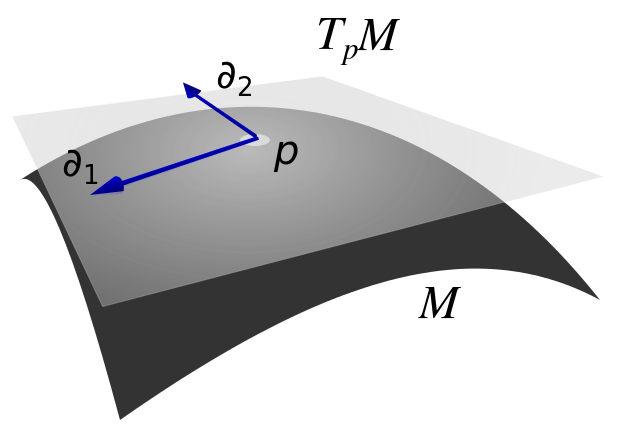
\includegraphics[scale=0.3]{Tangentialvektor.png}
	\caption{A visualisation of the tangent plane $T_{p} (M)$ to a manifold $M$ in 2 dimensions.}
\end{figure}

The vectors in the tangent space are what we will identify as contravariant vectors \cite{hartle, carroll}. Due to using the coordinate basis we can think of such vectors as being differential operators on the tangent plane. Thus we see that a vector can be represented as a sum of its coordinates \(A^{\mu}\) and the differential operators at the point \(\partial_{\nu}\). That is

\begin{equation} \label{contravariant}
	\vec{A} = A^{\mu} \partial_{\mu} = A^{0} \partial_{0} + A^{1} \partial_{1} + A^{2} \partial_{2} + A^{3} \partial_{3} .
\end{equation} 

We can now introduce another set of vectors at a point \(p\) on the manifold. If we consider the set of linear maps from the tangent space to the real numbers, \(\omega : T_{p} (M) \rightarrow \mathbb{R}\), we can construct the dual vector space of the tangent space to the manifold at a point \(p\), \(T_{p}^{*} (M)\) \cite{carroll}. We choose the basis of this vector space, \(\hat{e}^{\nu}\) such that \cite{carroll, hartle} 

\begin{equation} \label{cotangent-basis}
	\hat{e}^{\nu} \, \, \hat{e}_{\mu} = \df{\nu} (\partial_{\mu}) = \frac{\partial x^{\nu}}{\partial x^{\mu}} = \delta^{\nu}_{\mu} .
\end{equation} 

From this basis, \(\hat{e}^{\mu} = \df{\mu}\), we can construct any general linear map from vectors in the tangent space to the real numbers. Thus we can give an expression for the covectors much like \eqref{contravariant} \cite{carroll}

\begin{equation} \label{covarient}
	\vec{\omega} = \omega_{\mu} \df{\mu} = \omega_0 \df{0} + \omega_1 \df{1} +\omega_2 \df{2} +\omega_3 \df{3} .
\end{equation} 

Explicitly, by choosing the bases as we have, the linear mapping \(\omega : T_{p} (M) \rightarrow \mathbb{R}\) must be the same as the standard euclidean inner product \cite{hartle}. That is, if we take the contraction of a vector and a covector \(A^{\mu} \omega_{\mu}\) we obtain the sum of the product of the components of the vector and covector \cite{hartle}

\begin{equation} \label{inner}
	\begin{aligned}
	\omega_{\mu} \df{\mu} (A^{\nu} \partial_{\nu}) &= \omega_{\mu} A^{\nu} (\df{\mu} \partial_{\nu}) = \omega_{\mu} A^{\nu} \delta^{\mu}_{\nu} = \omega_{\mu} A^{\mu} \\
	&= \omega_0 A^0 + \omega_1 A^1 + \omega_2 A^2 + \omega_3 A^3 \in \mathbb{R} .
	\end{aligned}
\end{equation} 

From here on in we will refer to a vectors components, \(A^{\mu}\), as the vector itself, and the components of a covector as the covector itself. The implicit understanding here is that we are using the coordinate basis, and that therefore vectors at any point in the manifold will always be defined in the way given above.

We are now prepared to define the objects which we will use most throughout our discussion of General Relativity, tensors. First we recall a theorem from linear algebra.

\begin{thm} \label{dual}
In a finite dimensional vector space \(V\) with a dual space \(V^{*}\) the dual of the dual space \(V^{**}\) is isomorphic to the original space \(V\). {\normalfont\cite{szekeres}}
\end{thm}

Thus, due to \ref{dual}, we see that in addition to a covector acting on a vector as a linear operator we can consider the converse to be true: a vector can act on a covector as a linear operator. This is generally the case with a tensor: a tensor will take as an input vectors and covectors and map them to the real numbers. Thus we can define a tensor \(T\) as follows \footnote{In this definition we state that tensors map to the real numbers, however to be more correct we would have to say that tensors map to the field that the manifold is constructed over. Here we will always take this to be \(\mathbb{R}\).} \cite{carroll, szekeres}
\begin{equation} \label{tensor-def}
	T : \underbrace{T_{p}^{*}(M) \times \cdots \times T_{p}^{*}(M)}_{p \,\, \text{times}} \times \underbrace{T_{p}(M) \times \cdots \times T_{p}(M)}_{q \,\, \text{times}} \rightarrow \mathbb{R} .
\end{equation} 

In the above expression we take \(\times\) to be the Cartesian product: that is the above expression takes as an input ordered pairs of \(p\) covectors and \(q\) vectors.

We now can define the type of a tensor: the tensor above is of type \( \left[ \begin{smallmatrix} p \\ q \end{smallmatrix} \right] \). We will call the \(p\) covectors we input as \(p\) ``up'' indices and the \(q\) vectors ``down'' indices. That is, the tensor above would be given as \(T\indices{^{\sigma_{1}}^\cdots^{\sigma_{p}}_{\alpha_{1}}_\cdots_{\alpha_{q}}}\) \cite{carroll}. In this way we can see that vectors are a type \( \left[ \begin{smallmatrix} 1 \\ 0 \end{smallmatrix} \right] \) tensor and covectors are of type \( \left[ \begin{smallmatrix} 0 \\ 1 \end{smallmatrix} \right] \). We will define scalars to be of type \( \left[ \begin{smallmatrix} 0 \\ 0 \end{smallmatrix} \right] \) \cite{szekeres}. 

Finally we can introduce the tensor product, \(\otimes\). 
The tensor product is a linear product of tensors, that is if we add a tensor \(T\) of type \( \left[ \begin{smallmatrix} p \\ q \end{smallmatrix} \right] \) and a tensor \(S\) of type \( \left[ \begin{smallmatrix} r \\ s \end{smallmatrix} \right] \) we form \(T \otimes S\) of type \( \left[ \begin{smallmatrix} p+r \\ q+s \end{smallmatrix} \right] \). In terms of indices we have that the tensor product is like multiplication between tensors: if \(T = T^{\lambda \sigma}\) and \(S = S_{\mu \nu}\) then \(T \otimes S = T^{\lambda \sigma} S_{\mu \nu}\) \cite{carroll, szekeres}.

\subsection{Index Rules}

Before we continue it is worth summarizing the rules for index calculus with tensors. We use the Einstein summation convention throughout the text, where any repeated index (one upper and one lower) is summed over. That is, in an \(n\) dimensional space we would have 
\begin{equation} \label{summation-convention}
	v^i w_i = \sum_{i=0}^{n-1} v^i w_i
\end{equation}
assuming that we are using zero indexes. We can now introduce several other operations on tensors.
\begin{itemize}
	\item Contraction is an operation which maps a \( \left[ \begin{smallmatrix} p \\ q \end{smallmatrix} \right] \) type tensor to a \( \left[ \begin{smallmatrix} p-1 \\ q-1 \end{smallmatrix} \right] \) tensor by setting two of the indices equal to each other and summing them. That is if we have a tensor \( K\indices{^\mu^\lambda^\sigma_\alpha_\gamma_\phi}\) and we contract the \(\phi\) and \(\sigma\) indices we will obtain a new tensor, of type \( \left[ \begin{smallmatrix} 2 \\ 2 \end{smallmatrix} \right] \) \cite{carroll}
\end{itemize}
\begin{equation} \label{contration}
	K\indices{^\mu^\lambda^\sigma_\alpha_\gamma_\sigma} = \,\,\, L\indices{^\mu^\lambda_\alpha_\gamma} .
\end{equation}
\begin{itemize}
	\item[] In the case of a matrix this operation is the same as the trace. In order to contract over two upper or two lower indices we will need the metric tensor, which we will introduce in the next section.
	\item A tensor is considered to be symmetric in some of its indices if we can exchange their order and still obtain the same tensor. As an example, if \(S\indices{^\mu^\nu_\sigma_\alpha}\) is symmetric in the upper indices then \(S\indices{^\mu^\nu_\sigma_\alpha} = S\indices{^\nu^\mu_\sigma_\alpha}\) \cite{carroll}.
	\item Similarly a tensor is antisymmetric if when we exchange two indices we obtain the same tensor, but the tensor also changes sign. That is \(S\indices{^\mu^\nu_\sigma_\alpha} = -S\indices{^\nu^\mu_\sigma_\alpha}\).
	\item Given a tensor which is not symmetric we can create a symmetric tensor from it in any indices we wish. To do so we sum all permutations of the indices we are symmetrizing and divide by the number of terms in the sum. We will make clear which indices we are symmetrizing by surrounding them with round brackets \cite{carroll}
\end{itemize}
\begin{equation} \label{tensor-symmetrize}
	T\indices{_{(\mu_1 \mu_2 \cdots \mu_n)}_\rho^\sigma} = \frac{1}{n!} (T \indices{_{\mu_1}_{\mu_2}_{\cdots}_{\mu_n}_\rho^\sigma }
	+ \text{sum over permutations of indices}).
\end{equation}
\begin{itemize}
	\item In a similar way we can antisymmetrize a tensor in some of its indices using the same procedure, but alternating the sign of the terms in the sum over the permutations \cite{carroll}. We denote this by surrounding the relevant indices with square brackets.
\end{itemize}
\begin{equation} \label{tensor-antisymmetrize}
	T\indices{_{[\mu_1 \mu_2 \cdots \mu_n]}_\rho^\sigma} = \frac{1}{n!} (T \indices{_{\mu_1}_{\mu_2}_{\cdots}_{\mu_n}_\rho^\sigma }
+ \text{alternating sum over permutations of indices}) .
\end{equation}
\section{The Metric Tensor}

We now can define a new object on a manifold: the metric tensor \(g_{\mu \nu}\). This tensor is the ``star'' of General Relativity, as we will see in the subsequent discussion. From allowing us to perform calculations on the indices to allowing us to define the curvature of spacetime and eventually appearing in the all important Einstein Equation, the metric is omnipresent \cite{carroll, szekeres, cheng}.

We define the metric as being a type \( \left[ \begin{smallmatrix} 0 \\ 2 \end{smallmatrix} \right] \) tensor which takes two vectors as an input and gives back a separation between them
\begin{equation} \label{line-el}
	ds^2 = g_{\mu \nu} \df{\mu} \df{\nu} .
\end{equation}

Thus the metric supplies the idea of an inner product between two vectors, as opposed to a vector and a covector \cite{hartle}

\begin{equation} \label{inner-metric}
	g(\vec{A}, \vec{B}) = \vec{A} \cdot \vec{B} = g_{\mu \nu} A^{\mu} B^{\nu} .
\end{equation} 

We can now see how the metric must be used to raise and lower indices: in order for the inner product to work like \eqref{inner} we must have that the metric allows us to raise an index

\begin{equation} \label{raise}
	A_{\mu} = g_{\mu \nu} A^{\nu} .
\end{equation}

If we now introduce the inverse metric \(g^{\mu \nu}\) which is defined to be the tensor such that \cite{carroll}:
\begin{equation} \label{inverse-metric}
	g^{\mu \nu} g_{\nu \sigma} = g_{\lambda \sigma} g^{\lambda \mu} = \delta^{\mu}_{\sigma} \,\, ,
\end{equation}
\noindent we can then use the inverse metric to lower an index
\begin{equation} \label{lower}
	A^{\mu} = g^{\mu \nu} A_{\nu} .
\end{equation}

One of the most important features of relativistic theory is that \(ds^2\) must be a relativistic invariant, that is, no matter what choice of coordinates \(ds^2\) must always take the same value for the same spacetime events. We will see this is due to how tensors transform, with vectors transforming in such a way as to cancel the transformation of the matrix.

In the 4 dimensional spacetime of general relativity the metric takes the form of a position dependent symmetric 4 by 4 matrix with one negative and three positive eigenvalues 
\footnote{We can also take this to be one positive and three negative eigenvalues. The choice between the two is just convention.}. 
Explicitly, this is

\begin{equation} \label{metric-matrix}
	g_{\mu \nu} (x^{\sigma}) \equiv
	\begin{pmatrix} 
	g_{00} (x^{\sigma}) & g_{01} (x^{\sigma}) & g_{02} (x^{\sigma}) & g_{03} (x^{\sigma}) \\
	g_{01} (x^{\sigma}) & g_{11} (x^{\sigma}) & g_{12} (x^{\sigma}) & g_{13} (x^{\sigma}) \\
	g_{02} (x^{\sigma}) & g_{12} (x^{\sigma}) & g_{22} (x^{\sigma}) & g_{23} (x^{\sigma}) \\
	g_{03} (x^{\sigma}) & g_{13} (x^{\sigma}) & g_{23} (x^{\sigma}) & g_{33} (x^{\sigma}) 
\end{pmatrix} .
\end{equation}

\noindent In the special relativistic case where spacetime is flat this reduces to the Minkowski metric

\begin{equation} \label{metric-sr}
	\eta_{\mu \nu} (x^{\sigma}) \equiv
	\begin{pmatrix} 
	-1 & 0 & 0 & 0 \\
	0 & 1 & 0 & 0 \\
	0 & 0 & 1 & 0 \\
	0 & 0 & 0 & 1 
	\end{pmatrix} .
\end{equation}

In keeping with the equivalence principle it is also possible to transform the metric at any point such that is it the same as the Minkowski metric \(\eta_{\mu \nu}\) and that the first order partial derivatives vanish \cite{carroll}.

\section{Covariant Differentiation and the Connection}

In order to understand how to perform differentiation on the manifold we first need to understand how tensors transform from one coordinate system to another in general.

\noindent If we wish to switch from one set of coordinates $x^{\mu}$ to a new set of coordinates $x^{\mu^\prime}$. We define the matrix of transformation between the coordinates for a vector as \cite{cheng}

\begin{equation} \label{vector-transform}
	A^{\mu} \rightarrow A^{\mu^\prime} = \frac{\partial x^{\mu^\prime}}{\partial x^{\mu}} A^{\mu} .
\end{equation}

For a covector we have \cite{cheng}
\begin{equation} \label{covector-transform}
	A_{\mu} \rightarrow A_{\mu^\prime} = \frac{\partial x^{\mu}}{\partial x^{\mu^\prime}} A_{\mu} .
\end{equation}

Now we can define the transformation for an arbitrary tensor \footnote{We can consider this tensor transformation as another way of defining tensors, that is that they are objects which transform linearly under coordinate transformations.} \cite{carroll}
\begin{equation} \label{tensor-transform}
	T\indices{^{\mu_1}^{\cdots}^{\mu_k}_{\nu_1}_{\cdots}_{\nu_l}} \rightarrow T\indices{^{\mu_1^\prime}^{\cdots}^{\mu_k^\prime}_{\nu_1^\prime}_{\cdots}_{\nu_l^\prime}}
	= \frac{\partial x^{\mu_1^\prime}}{\partial x^{\mu}} \cdots \frac{\partial x^{\mu_k^\prime}}{\partial x^{\mu_k}} \frac{\partial x^{\nu_1}}{\partial x^{\nu_1^\prime}} \cdots 
	\frac{\partial x^{\nu_l}}{\partial x^{\nu_l^\prime}}
	T\indices{^{\mu_1}^{\cdots}^{\mu_k}_{\nu_1}_{\cdots}_{\nu_l}} .
\end{equation}

Now we can consider partial derivatives. The partial derivative operator is a covector, as shown in \eqref{coordinate-basis}, and transforms in the same way as any other covector given in \eqref{covector-transform}. However, when we apply the derivative to a vector and then attempt to change coordinates the result does not follow the rules. To see this consider $\partial_{\nu^\prime} A^{\mu^\prime}$ the derivative of a vector field. Use the definition \eqref{vector-transform} and differentiate on both sides \cite{cheng}
\begin{equation} \label{partial-transform}
\begin{aligned}
	\partial_{\nu^\prime} A^{\mu^\prime} &= \frac{\partial}{\partial x^{\nu^\prime}} \left(\frac{\partial x^{\mu^\prime}}{\partial x^{\rho}} A^{\rho}\right) \\
	&= \frac{\partial x^{\lambda}}{\partial x^{\nu^\prime}} \frac{\partial x^{\mu^\prime}}{\partial x^{\rho}} (\partial_{\lambda} A^{\rho}) + \frac{\partial^2 x^{\mu^\prime}}{\partial x^{\nu^\prime} \partial x^{\rho}} A^{\rho}
\end{aligned}
\end{equation}
which is not the same as the tensor transformation law given in \eqref{tensor-transform}.

This discrepancy is due to the position dependent transformation of tensors. Since on an arbitrary manifold the basis vectors of the tangent plane at a point are dependent on the choice of coordinate system, a tensor defined at one point will not necessarily be the same at another point \cite{cheng}.

In order to solve this problem we must introduce a new type of derivative which will transform as we expect under coordinate transformations. This is the covariant derivative. In order to find the covariant derivative we must first list several of the properties we will expect it to have \cite{carroll}.

\begin{itemize}
	\item Linearity: \(\nabla (T + S) = \nabla T + \nabla S\) .
	\item Obeys the product rule: \(\nabla (T \otimes S) = (\nabla T) \otimes S + T \otimes (\nabla S)\) .
	\item Commutes with the contraction operation: \(\nabla_{\mu} (S\indices{^\lambda_\lambda_\rho}) = (\nabla S)\indices{_\mu^\lambda_\lambda_\rho}\) .
	\item Like the partial derivative it maps a \( \left[ \begin{smallmatrix} r \\ s \end{smallmatrix} \right] \) type tensor to a \( \left[ \begin{smallmatrix} r \\ s+1 \end{smallmatrix} \right] \) type tensor.
	\item For a scalar, the covariant derivative is the same as a the partial derivative \(\nabla_{\mu} \phi = \partial_{\mu} \phi\).
\end{itemize}

In order for the operation to follow the product rule we will require it to be the same as the partial derivative plus an additional linear correction term \cite{carroll}. In order to do this we introduce a new linear term in the derivative, called the connection coefficients, which make the transformation of a derivative occur in the tensorial way. These coefficients are viewed as a matrix for each of the coordinate functions, that is \((\Gamma_{\mu})\indices{^\rho_\sigma}\) \cite{carroll}. We will drop the use of the brackets and understand that \(\Gamma^{\nu}_{\mu \sigma}\) has the same meaning. The covariant derivative of a vector will now be
\begin{equation} \label{co-deriv}
	\nabla_{\mu} V^{\nu} = \partial_{\mu} V^{\nu} + \Gamma^{\nu}_{\mu \sigma} V^{\sigma} .
\end{equation}

The transformation of this expression is designed to be tensorial, and as such the connection coefficients will not transform in a tensorial way but will transform so as to make the overall transformation tensorial. The transformation of the coefficients will be as follows \cite{carroll}: 

\begin{equation} \label{connection-transform}
	\Gamma^{\nu}_{\mu \sigma} \rightarrow \Gamma^{\nu'}_{\mu' \sigma'} = \frac{\partial x^{\mu}}{\partial x^{\mu'}} 
	\frac{\partial x^{\sigma}}{\partial x^{\sigma'}} \frac{\partial x^{\nu'}}{\partial x^{\nu}} \Gamma^{\nu}_{\mu \sigma} +
	\frac{\partial x^{\mu}}{\partial x^{\mu'}} \frac{\partial x^{\sigma}}{\partial x^{\sigma'}} \frac{\partial^2 x^{\nu'}}{\partial x^{\mu} \partial x^{\sigma}}
	.
\end{equation}

This will now correct for the second term in the expansion of the partial derivative of a vector, making it tensorial. In order to find the covariant derivative of a covector we first consider the derivative of the scalar \(\omega_{\mu} A^{\mu}\) \cite{carroll}. The definition of the covariant derivative given above is only for vectors, however it is reasonable to assume that the covariant derivative for a covector will be similar. Thus we introduce a new coefficient, which we will call \(\xi^{\sigma}_{\mu \lambda}\) for now, and covariantly differentiate \(\omega_{\mu} A^{\mu}\):

\begin{equation} \label{covar-deriv}
	\begin{aligned}
		\nabla_{\mu} (\omega_{\lambda} A^{\lambda}) &= (\nabla_{\mu} \omega_{\lambda}) A^{\lambda} + \omega_{\lambda} (\nabla_{\mu} A^{\lambda}) \\
		&= (\partial_{\mu} \omega_{\lambda}) A^{\lambda} + \xi^{\sigma}_{\mu \lambda} \omega_{\sigma} A^{\lambda}
		+ \omega_{\lambda} (\partial_{\mu} A^{\lambda}) + \omega_{\lambda} \Gamma^{\lambda}_{\mu \rho} A^{\lambda} .
	\end{aligned}
\end{equation}

Since this is the covariant derivative of a scalar, we must have that it is equal to the partial derivative. Thus we can also write:

\begin{equation} \label{covar-partial}
	\begin{aligned}
		\nabla_{\mu} (\omega_{\lambda} A^{\lambda}) &= \partial_{\mu} (\omega_{\lambda} A^{\lambda}) \\
		&= (\partial_{\mu} \omega_{\lambda}) A^{\lambda} + \omega_{\lambda} (\partial_{\mu} A^{\mu}) .
	\end{aligned}
\end{equation}

From here we can obviously see that \(\xi^{\sigma}_{\mu \lambda} = - \Gamma^{\lambda}_{\mu \rho}\) and thus for a covector the covariant derivative is given by \cite{carroll}

\begin{equation} \label{covar-diff}
	\nabla_{\mu} \omega_{\nu} = \partial_{\mu} \omega_{\nu} - \Gamma^{\lambda}_{\mu \nu} \omega_{\lambda} .
\end{equation}

We can now define the covariant derivative for any tensor, once again by considering it as a product of vectors and covectors, thus we see \cite{carroll}

\begin{equation} \label{tensor-diff}
	\begin{aligned}
	\nabla_{\sigma} T\indices{^{\mu_1}^\cdots^{\mu_k}_{\nu_1}_\cdots_{\nu_l}} = \partial_{\sigma} T\indices{^{\mu_1}^\cdots^{\mu_k}_{\nu_1}_\cdots_{\nu_l}}
	&+ \Gamma^{\mu_1}_{\sigma \lambda} T\indices{^{\mu_1}^\cdots^{\mu_k}_{\nu_1}_\cdots_{\nu_l}} + \, \cdots \, + \Gamma^{\mu_k}_{\sigma \lambda} T\indices{^{\mu_1}^\cdots^{\mu_k}_{\nu_1}_\cdots_{\nu_l}} \\
	&- \Gamma^{\lambda}_{\sigma \nu_1} T\indices{^{\mu_1}^\cdots^{\mu_k}_{\nu_1}_\cdots_{\nu_l}} - \, \cdots \, - \Gamma^{\lambda}_{\sigma \nu_l} T\indices{^{\mu_1}^\cdots^{\mu_k}_{\nu_1}_\cdots_{\nu_l}} .
	\end{aligned}
\end{equation}

Now we can introduce the specific connection we will use in General Relativity, the Levi-Civita connection \cite{carroll, szekeres}. With this connection we demand the following things:

\begin{itemize}
	\item The connection coefficients are torsion free, that is \(\Gamma^{\lambda}_{\mu \nu} = \Gamma^{\lambda}_{\nu \mu}\).
	\item Metric compatibility, that is \(\nabla_{\mu} g_{\nu \sigma} = 0\).
\end{itemize}

The Levi-Civita connection is the only connection which will have both such properties. This is known as the fundamental theorem of Riemannian geometry. From here we can derive an expression for the connection coefficients for the Levi-Civita connection in terms of the metric. If we consider the covariant derivative of the metric \(\nabla_{\rho} g_{\mu \nu}\) and permute the three indices \cite{carroll, cheng}:

\begin{equation} \label{metric-deriv}
	\begin{aligned}
		\nabla_{\rho} g_{\mu \nu} &= \partial_{\rho} g_{\mu \nu} - \Gamma^{\lambda}_{\rho \mu} g_{\lambda \nu} - \Gamma^{\lambda}_{\rho \nu} g_{\mu \nu} = 0 ,\\
		\nabla_{\mu} g_{\nu \rho} &= \partial_{\mu} g_{\nu \rho} - \Gamma^{\lambda}_{\mu \nu} g_{\lambda \rho} - \Gamma^{\lambda}_{\mu \rho} g_{\nu \lambda} = 0 ,\\
		\nabla_{\nu} g_{\rho \mu} &= \partial_{\nu} g_{\rho \mu} - \Gamma^{\lambda}_{\nu \rho} g_{\lambda \mu} - \Gamma^{\lambda}_{\nu \mu} g_{\rho \lambda} = 0 .
	\end{aligned}
\end{equation}

Now if we take the first equation and subtract the second and third from it, then multiply by the inverse metric we will obtain the desired expression for the coefficients \cite{carroll}

\begin{equation} \label{christ-def}
	\Gamma^{\lambda}_{\mu \nu} = \frac{1}{2} g^{\lambda \sigma} \left( \partial_{\mu} g_{\nu \sigma} + \partial_{\nu} g_{\sigma \mu} - \partial_{\sigma} g_{\mu \nu} \right) .
\end{equation}

This is the expression we will use as the definition of the connection coefficients.

\section{Parallel Transport}

In order to understand the curvature on the manifold we first need a new concept called parallel transport. Parallel transport is the operation of moving a tensor along a path on the manifold in such a way that the covariant derivative of the tensor along the path is zero. That is any changes to the tensor as a result of moving along the curve are due to the structure of space, not due to the tensor itself changing.

If we consider a curve \(\gamma\) on the manifold \(M\) given by a parameterization \(x^{\mu} (\lambda)\) with \(\lambda\) an affine parameter \footnote{An affine parameter is a parameter which is related to the proper time \(\tau\) by real coefficients \(a\) and \(b\) in the form \( \lambda = a \tau + b\). We will introduce the proper time soon.} and with the tangent vector to the curve of \(T^{\mu} = \frac{d x^{\mu}}{d \lambda}\) we can define the directional covariant derivative to be \cite{carroll}

\begin{equation} \label{directional}
	\frac{D}{d \lambda} = \frac{d x^{\mu}}{d \lambda} \nabla_{\mu} .
\end{equation}

We now say that a vector \(V^{\mu}\) is parallel transported along \(\gamma\) when

\begin{equation} \label{parallel}
	\frac{D V^{\mu}}{d \lambda} = 0 .
\end{equation}

This can be rephrased as \cite{carroll}

\begin{equation} \label{vector-parallel}
	\frac{d}{d \lambda} V^{\mu} + \Gamma^{\mu}_{\sigma \rho} \frac{d x^{\sigma}}{d \lambda} V^{\rho} = 0 .
\end{equation}

We are now ready to define one of the key ideas in general relativity: a geodesic path. A geodesic is the shortest path between two points, and brings the idea of a straight line in flat space into the curved spaces we will use in relativity. In keeping with this idea, we will define a geodesic to be a path for which the tangent vector \(T^{\mu}\) is parallel transported along the path \cite{carroll}. That is

\begin{equation} \label{geodesic0}
	\frac{D}{d \lambda} T^{\mu} = \frac{D}{d \lambda} \frac{d x^{\mu}}{d \lambda} = 0 .
\end{equation}

Inserting this into \eqref{vector-parallel} gives the standard geodesic equation: 

\begin{equation} \label{geodesic}
	\frac{d^2 x^{\mu}}{d \lambda^2} + \Gamma^{\mu}_{\rho \sigma} \frac{d x^{\rho}}{d \lambda} \frac{d x^{\sigma}}{d \lambda} = 0 .
\end{equation}

These results can also be obtained using variational methods \cite{carroll}, however we will not reproduce such proofs here. 

\section{World Lines}

A world line is a path \(\gamma\) as measured on the spacetime manifold between events. We can then define the type of the world line by considering what physical phenomena can occur on that path through spacetime. Since the speed of light is the highest attainable speed we will find that spacetime intervals can be divided into cases where normal objects can traverse the distance in spacetime, only light can traverse the distance in spacetime, or no physical phenomena can travserse the distance \cite{cheng, hartle, carroll}. 

We have, for the tangent vector \(T^{\mu}\) to a curve \(\gamma\) with parameter \(\lambda\) the following three possibilities:

\begin{itemize}
	\item If \(g_{\mu \nu} T^{\mu} T^{\nu} = 0\) then the curve is light-like or null. Paths such as these are the paths which light travels along.
	\item If \(g_{\mu \nu} T^{\mu} T^{\nu} < 0\) then the curve is time-like. These paths are the paths which objects with mass travel along, at less than the speed of light.
	\item If \(g_{\mu \nu} T^{\mu} T^{\nu} > 0\) then the curve is space-like. These paths are impossible for any object to travel along, and thus are completely physically disparate.
\end{itemize}

If we choose the parameterization of the curve \(\gamma\) such that \(g_{\mu \nu} T^{\mu} T^{\nu} = -1\) then the parameter is the proper time for an object, \(\tau\). This is the time measured by an observer moving on the path \(\gamma\) through spacetime \cite{cheng}.

For a timelike path we can now rewrite the geodesic equation \eqref{geodesic} in terms of the four-velocity \cite{carroll} \(U^{\mu} = dx^{\mu} / d \tau\)

\begin{equation} \label{geodesic-timelike}
	U^{\nu} \nabla_{\nu} U^{\mu} = 0 .
\end{equation}

\section{Riemann Curvature Tensor}

In order to measure the curvature of a manifold we need a new tensor which measures the change of a vector moving on the manifold around a closed loop. We choose a closed loop in order to see how the manifold varies from flat space: if the vector is unchanged by its journey around the loop then we should be in flat space \cite{cheng, carroll}.

For an arbitrary vector \(V^{\mu}\) we have that the Riemann curvature tensor is defined as \cite{carroll}

\begin{equation} \label{riemann}
	(\nabla_{\phi} \nabla_{\sigma} - \nabla_{\sigma} \nabla_{\phi}) V^{\mu} = R\indices{^\mu_\nu_\phi_\sigma} V^{\nu} .
\end{equation}

This definition of the Riemann curvature tensor is only true for connections which have torsion free coefficients \cite{lovelock}.

While we will not prove this definition, we can give some motivation for how it works. The covariant derivative effectively measures how much a vector moves away from a path on which it is parallel transported. On flat space, this deviation would be zero, and thus the curvature tensor would be zero. The terms involving the covariant derivative measure the change of a vector compared to its parallel transport in that direction. Thus by considering two different directions we can obtain the loop mentioned above. This also gives the condition that in flat space the tensor should be zero, as \(\nabla_{\phi} \nabla_{\sigma} - \nabla_{\sigma} \nabla_{\phi} = \partial_{\phi} \partial_{\sigma} - \partial_{\sigma} \partial_{\phi} = 0\) in flat space \cite{cheng, carroll, woodhouse}.

If we now perform the computation in \eqref{riemann} with an arbitrary vector \(V^{\lambda}\) we can obtain an expression for the Riemann curvature tensor in terms of the connection coefficients \cite{carroll, woodhouse}. First consider \(\nabla_{\mu} \nabla_{\nu} V^{\lambda}\)

\begin{equation} \label{riemann-deriv}
	\begin{aligned}
		\nabla_{\mu} \nabla_{\nu} V^{\lambda} &= \nabla_{\mu} (\partial_{\nu} V^{\lambda} + \Gamma^{\lambda}_{\nu \sigma} V^{\sigma}) \\
		&= \partial_{\mu} \partial_{\nu} V^{\lambda} + (\partial_{\mu} \Gamma^{\lambda}_{\nu \sigma}) + \Gamma^{\lambda}_{\nu \sigma} \partial_{\mu} V^{\sigma}
		+ \Gamma^{\lambda}_{\mu \phi} (\partial_{\nu} V^{\phi} + \Gamma^{\phi}_{\nu \sigma} V^{\sigma}) - \Gamma^{\sigma}_{\mu \nu} (\partial_{\sigma} V^{\lambda}
		+ \Gamma^{\lambda}_{\phi \sigma})
	\end{aligned}
\end{equation}
now by exchanging \(\mu\) and \(\nu\) and using the properties of the connection we can find
\begin{equation} \label{riemann-deriv2}
	(\nabla_{\mu} \nabla_{\nu} - \nabla_{\nu} \nabla_{\mu}) V^{\lambda} = (\partial_{\mu} \Gamma^{\lambda}_{\nu \sigma} - \partial_{\nu}\Gamma^{\lambda}_{\mu \sigma} 
	+ \Gamma^{\lambda}_{\mu \lambda} \Gamma^{\phi}_{\nu \sigma} - \Gamma^{\lambda}_{\nu \lambda} \Gamma^{\phi}_{\mu \sigma}) V^{\sigma} .
\end{equation}

Thus we can give an expression for the Riemann curvature tensor in terms of the connection coefficients. This is the expression most commonly used to calculate the tensor 

\begin{equation} \label{riemann-christoffel}
	R\indices{^\rho_\sigma_\mu_\nu} = \partial_{\mu} \Gamma^{\rho}_{\nu \sigma} - \partial_{\nu}\Gamma^{\rho}_{\mu \sigma} 
	+ \Gamma^{\rho}_{\mu \lambda} \Gamma^{\lambda}_{\nu \sigma} - \Gamma^{\rho}_{\nu \lambda} \Gamma^{\lambda}_{\mu \sigma} .
\end{equation}

\subsection{Properties of the Riemann Curvature Tensor}

We will list some of the important properties of the Riemann curvature tensor. These are easier to see in the version of the tensor with 4 lower indices 

\begin{equation} \label{riemann-lower}
	R\indices{_\rho_\sigma_\mu_\nu} = g_{\rho \lambda} R\indices{^\lambda_\sigma_\mu_\nu} .
\end{equation}

\begin{itemize}
	\item Antisymmetry in the first two indices \(R\indices{_\rho_\sigma_\mu_\nu} = -R\indices{_\sigma_\rho_\mu_\nu}\) and in the last two indices \\ \(R\indices{_\rho_\sigma_\mu_\nu} = -R\indices{_\rho_\sigma_\nu_\mu}\).
	\item Symmetric when exchanging the first pair of indices with the second \(R\indices{_\rho_\sigma_\mu_\nu} = R\indices{_\mu_\nu_\rho_\sigma}\).
	\item The sum of the cyclic permutations of the last three indices is zero \(R\indices{_\rho_\sigma_\mu_\nu} + R\indices{_\rho_\mu_\nu_\sigma} + R\indices{_\rho_\nu_\sigma_\mu} = 0\)
\end{itemize}

From these properties it is possible to show that in \(n\) dimensional space the Riemann curvature tensor must have \(N\) independent components \cite{cheng}, where \(N\) is
\begin{equation}
	N = \frac{1}{12} n^2 (n^2 -1) .
\end{equation}

\begin{remark}
When \(n=1\) we have that \(N = 0\) and thus there can be no curvature for a line. For a surface however, with \(n=2\), we find that \(N=1\). This single independent component is related to the Gaussian curvature {\normalfont \cite{cheng, landau}} of a surface from classical differential geometry. We have that
\begin{equation}
	K = - \frac{R_{1212}}{|g_{\mu \nu}|}
\end{equation}
with \(|g_{\mu \nu}|\) being the determinant of the metric tensor and \(K\) the Gaussian curvature. With \(n=4\) we have 20 independent components of the Riemann curvature tensor.
\end{remark}

Finally another important property is the Bianchi identity

\begin{equation} \label{bianchi}
	\nabla_{\omega} R\indices{_\rho_\sigma_\mu_\nu} + \nabla_{\rho} R\indices{_\sigma_\omega_\mu_\nu} + \nabla_{\sigma} R\indices{_\omega_\rho_\mu_\nu} = 0 .
\end{equation}

We can also write this by using the antisymmetry properties of \(R\indices{_\rho_\sigma_\mu_\nu}\) as

\begin{equation} \label{bianchi2}
	\nabla_{[\omega} R\indices{_\rho_{\sigma ]}_\mu_\nu} = 0 .
\end{equation}

\subsection{Ricci Tensor}

If we now contract the first and third indices of the Riemann curvature tensor we can form the Ricci tensor \cite{carroll}

\begin{equation} \label{ricci-tensor}
	R\indices{_\mu_\nu} = R\indices{^\lambda_\mu_\lambda_\nu} .
\end{equation}

Due to our choice of the connection this is the only contraction of the Riemann curvature tensor which yields interesting results. All other contractions are either zero or related to the Ricci tensor \cite{carroll}. The Ricci tensor is also symmetric in its indices.

\subsection{Ricci Scalar}

If we now raise one of the indices of the Ricci tensor and then contract over the indices we will obtain the Ricci scalar

\begin{equation} \label{ricci-scalar}
	R = R\indices{^\mu_\mu} = g^{\mu \nu} R_{\mu \nu} .
\end{equation}

\subsection{Einstein Tensor}

We now can derive the Einstein tensor, which is the tensor we will use to describe the curvature of space in the Einstein equation. If we take the Bianchi identity \eqref{bianchi} and contract twice we will obtain a similar identity in terms of the Ricci tensor and scalar

\begin{equation} \label{bianchi-contract}
	\begin{aligned}
		g^{\nu \sigma} g^{\mu \lambda} (\nabla_{\lambda} R\indices{_\rho_\sigma_\mu_\nu} + \nabla_{\rho} R\indices{_\sigma_\lambda_\mu_\nu} + \nabla_{\sigma} R\indices{_\lambda_\rho_\mu_\nu}) &= 0  , \\
		\nabla^{\mu} R\indices{_\rho_\mu} - \nabla_{\rho} R + \nabla^{\nu} R\indices{_\rho_\nu} &= 0 .
	\end{aligned}
\end{equation}

\noindent Now if we define the Einstein tensor 
\begin{equation} \label{einstein-tensor}
	G\indices{_\mu_\nu} = R\indices{_\mu_\nu} - \frac{1}{2} R g_{\mu \nu}
\end{equation}
we can see that the contracted Bianchi identity must imply that \cite{cheng, carroll}
\begin{equation} \label{etensor0}
	\nabla^{\mu} G\indices{_\mu_\nu} = 0 .
\end{equation}

\section{The Energy Momentum Tensor}

The fundamental idea of General Relativity is that the curvature of spacetime is caused by the nearby mass and energy at that point \cite{hartle, carroll}. We now have the mathematical description of how the curvature of space is measured. Thus, we now need to develop an object to measure the amount of mass and energy near a point. This is the energy momentum tensor.

The energy momentum tensor is a type \( \left[ \begin{smallmatrix} 2 \\ 0 \end{smallmatrix} \right] \) symmetric tensor which measures the flux of four momentum \(p^{\mu}\) across a surface keeping one coordinate constant \cite{carroll}. In 3 dimensional flat space this would represent the forces pointing in three orthogonal directions along three orthogonal planes at a point \cite{cheng}.

In 4 dimensional general relativity we have to take into account energy as well, as due to the classic equation from special relativity for the rest energy of matter
\begin{equation} \label{ifweonlyhadoneequation}
	E = mc^2
\end{equation}
we can view energy as having a mass. Thus in the 4 dimensional case we take the energy momentum tensor to be in matrix form
\begin{equation} \label{e-m-tensor}
	T^{\mu \nu} = 
	\begin{pmatrix} 
		T^{00} & T^{01} & T^{02} & T^{03} \\ 
		T^{10} & T^{11} & T^{12} & T^{13} \\ 
		T^{20} & T^{21} & T^{22} & T^{23} \\ 
		T^{30} & T^{31} & T^{32} & T^{33} 
	\end{pmatrix} .
\end{equation}

We can now identify the components of this equation \cite{hartle, carroll}

\begin{itemize}
	\item \(T^{00}\) is the energy density at the point, which we will call \(\rho\). 
	\item \(T^{0i} = T^{i0}\) for the three spatial indices is the momentum density at the point.
	\item Terms on the diagonal \(T^{ii}\) give the spatial components of the pressure \(p_{i}\).
	\item All other off diagonal terms represent the sheering terms, that is forces on the planes not in the direction of the plane. These are created due to things like viscosities.
\end{itemize}

An example of this, and the one used most in modeling physical situations in general relativity is of the perfect fluid, which we will take to have an energy momentum tensor of \cite{carroll, hartle}
\begin{equation} \label{perfect-fluid}
	T^{\mu \nu} = 
	\begin{pmatrix}
	\rho & 0 & 0 & 0 \\
	0 & p & 0 & 0 \\
	0 & 0 & p & 0 \\
	0 & 0 & 0 & p
	\end{pmatrix}
\end{equation}
in the rest frame of the fluid. We now give a tensorial version of this equation which is valid in any frame \cite{carroll}
\begin{equation} \label{perfect-fluid-tensor}
	T^{\mu \nu} = (\rho + p) U^{\mu} U^{\nu} + p g^{\mu \nu}
\end{equation}
where we define \(U^{\mu}\) to be the constant four velocity of the particles within the fluid. 

Another important property of the energy momentum tensor is that it must be conserved, that is
\begin{equation} \label{e-m-conversed}
	\nabla_{\mu} T^{\mu \nu} = 0 .
\end{equation}
This is related to the conservation of energy and momentum in an inertial frame \cite{carroll, hartle}.

\section{The Einstein Equation}

At its core, general relativity is about relating the curvature of spacetime to the matter distribution in space. This is illustrated by the Einstein equation \cite{carroll, hartle}

\begin{equation} \label{einstein-eqn}
	G_{\mu \nu} = k T_{\mu \nu} 
\end{equation}
for some constant \(k\) which we will soon find. The Einstein equation is the field equation for general relativity, describing exactly how the curvature of spacetime happens due to the presence of mass.

Our choice of the Einstein tensor in this equation is due to requiring a tensor based on the curvature but always having a zero covariant derivative. We see the latter from \eqref{etensor0}, and the former is due to derivation of the Einstein tensor in terms of the Riemann curvature tensor and eventually the metric.

In order to find the constant \(k\) of proportionality between the two tensors we recall the field equation for Newtonian gravity

\begin{equation} \label{poisson}
	\nabla^2 \Phi = 4\pi G \rho .
\end{equation}

\noindent In the case of a weak gravitational field, we must have that Einstein's gravitational theory reduces to the Newtonian theory.

If we contract \eqref{einstein-eqn} on both sides we will obtain \cite{carroll, cheng}
\begin{equation} \label{einstein-contract}
	R = - k T
\end{equation}
which we can use to rewrite \eqref{einstein-eqn} as
\begin{equation} \label{einstein-eqn2}
	R_{\mu \nu} = k \left(T_{\mu \nu} - \frac{1}{2} T g_{\mu \nu}\right) .
\end{equation}

We now need to see how to recover Newton's theory of gravitation for weak gravitational fields and slowly moving objects. In a weak field case, we will be able to assume that spacetime is mostly flat like 4 dimensional Minkowski space and the metric will be \(\eta_{\mu \nu}\) other than a small perturbation, which we will call \(h_{\mu \nu}\) \cite{carroll, woodhouse}. We can now decompose a weak field metric into components
\begin{equation} \label{weak-field}
	g_{\mu \nu} = \eta_{\mu \nu} + h_{\mu \nu}
\end{equation}
with \(|h_{\mu \nu}| << 1\). Due to taking the determinant of \(h_{\mu \nu}\) to be very small, we will ignore products of \(h_{\mu \nu}\) with itself. Thus to first order we can find the inverse metric
\begin{equation} \label{weak-field-inverse}
	g^{\mu \nu} = \eta^{\mu \nu} - h^{\mu \nu}
\end{equation}
where we now use the Minkowski metric to raise and lower indices.

If we also assume that any objects with mass are moving at much less than the speed of light, then we can say for the three spacial coordinates \(x^i\) and the time coordinate \(t\) that in terms of the proper time \(\tau\) \cite{carroll}
\begin{equation} \label{slow-moving}
	\frac{d x^i}{d \tau} << \frac{d t}{d \tau} .
\end{equation}
As such, we can simplify the geodesic equation by assuming that terms involving the slowly changing spatial coordinates do not make a large difference to the path, and write
\begin{equation} \label{slow-moving-geodesic}
	\frac{d x^{\mu}}{d \tau^2} + \Gamma^{\mu}_{00} \left( \frac{d t}{d \tau} \right)^2 = 0 .
\end{equation}

In Newtonian gravity we would also have that the field is time independent, thus, we can take that \(\partial_{0} g_{\mu \nu} = 0\) and therefore compute the connection coefficients for this weak field. Due to \eqref{slow-moving-geodesic} we only need calculate the connection coefficent corresponding to the time coordinate
\begin{equation} \label{coefficent-weak}
	\begin{aligned}
	\Gamma^{\mu}_{00} &= \frac{1}{2} g^{\mu \lambda} (\partial_0 g_{\lambda 0} + \partial_0 g_{0 \lambda} - \partial_{\lambda} g_{00}) \\
	&= - \frac{1}{2} g^{\mu \lambda} \partial_{\lambda} g_{00} .
	\end{aligned}
\end{equation}

In the case of \eqref{weak-field} we have, to first order in \(h_{\mu \nu}\) \cite{carroll}
\begin{equation} \label{coefficent-weak2}
	\Gamma^{\mu}_{00} = - \frac{1}{2} \eta^{\mu \lambda} \partial_{\lambda} h_{00}
\end{equation}
and thus we can rewrite the geodesic equation \eqref{slow-moving-geodesic}
\begin{equation} \label{geodesic-connections-slow}
	\frac{d^2 x^{\mu}}{d \tau^2} = \frac{1}{2} \eta^{\mu \lambda} \partial_{\lambda} h_{00} \left( \frac{d t}{d \tau} \right)^2 .
\end{equation}

If we now recall the special relativistic result that \(\frac{d t}{d \tau} = \gamma\) then in the slow moving frame \(\gamma \approx 1\), and thus we can use the time coordinate \(t\), as \(t\) and \(\tau\) will coincide. Therefore
\begin{equation} \label{geodesic-connections-slow2}
	\frac{d^2 x^{\mu}}{d t^2} = \frac{1}{2} \eta^{\mu \lambda} \partial_{\lambda} h_{00} .
\end{equation}

If we now consider just the spatial coordinates, then \(\eta^{\mu \nu} = \delta\indices{^\mu_\nu}\) for 3 dimensional flat space. Thus, we can write, with \(i\) from 1 to 3
\begin{equation} \label{nearly-newtonian}
	\frac{d^2 x^i}{d t^2} = \frac{1}{2} \partial_{i} h_{00} .
\end{equation}

Now if we recall that the acceleration due to a gravitational potential \(\Phi\) in Newtonian gravity is \(a = - \nabla \Phi\) then we see that \eqref{nearly-newtonian} is in the same form, if we choose \(h_{00} = - 2 \Phi\). This is then equivalent to choosing the first coefficient of the metric as \cite{carroll}
\begin{equation} \label{metric-newtonian}
	g_{00} = - (1 + 2 \Phi) .
\end{equation}

Finally, let us consider a collection of dust, that is a collection of particles for which the energy momentum tensor is \(T_{\mu \nu} = \rho U_{\mu} U_{\nu}\) (this is the case of \eqref{perfect-fluid-tensor} without pressure) and we consider the inertial frame where \(U^{\mu} = (1, 0, 0, 0)\). Then we will have that \cite{carroll, cheng}
\begin{equation} \label{dust-emt}
	T_{00} = \rho
\end{equation}
and all other coefficients will be zero. The trace of this energy momentum will be \(T = g^{00} T_{00} = - \rho\) and thus we can insert these into \eqref{einstein-eqn2} to gain an approximation for \(k\).

\begin{equation} \label{einstein-equation-newtonian}
	\begin{aligned}
		R_{00} &= k \left( T_{00} - \frac{1}{2} T g_{00}\right) \\
		&= \frac{1}{2} k \rho
	\end{aligned}
\end{equation}
since we are taking that \(g_{00} \approx \eta_{00} = -1\) in the Newtonian limit. If we now consider the definition of the Ricci tensor in terms of the Riemann curvature tensor we can obtain an approximate expression in terms of the metric and its perturbation as in \eqref{weak-field}
\begin{equation} \label{riemann-weak}
	 R_{00} = R\indices{^i_0_j_0} = \partial_{j} \Gamma^{i}_{00} - \partial_{0} \Gamma^{i}_{j0} + \Gamma^{i}_{j\lambda} \Gamma^{\lambda}_{00} - \Gamma^{i}_{0\lambda} \Gamma^{\lambda}_{j0}
\end{equation}
with \(i\) and \(j\) running from 1 to 3 \cite{carroll}. If we now note that products of \(\Gamma\) are products of the metric perturbation and are therefore very small we can ignore these in the Newtonian limit. Also, the time derivative \(\partial_{0}\) is automatically zero due to the static field. Thus we must have that the Riemann curvature tensor in the form \(R\indices{^i_0_j_0} = \partial_{j} \Gamma^{i}_{00}\) and if we now use \eqref{coefficent-weak2} we can calculate 
\begin{equation} \label{soclose}
	\begin{aligned}
		R_{00} &= - \frac{1}{2} \delta^{ij} \partial_i \partial_j h_{00} \\
		&= - \frac{1}{2} \nabla^2 h_{00} .
	\end{aligned}
\end{equation}

Thus we can write
\begin{equation} \label{icantasteit}
	\nabla^2 h_{00} = - k \rho .
\end{equation}

However since we set \(h_{00} = -2\Phi\) as in \eqref{metric-newtonian} we recover Poisson's equation \eqref{poisson} when we set \(k = 8 \pi G\). Thus, we can give the correct expression for the Einstein equation

\begin{equation} \label{einstein-right}
	R_{\mu \nu} - \frac{1}{2} R g_{\mu \nu} = 8 \pi G T_{\mu \nu} .
\end{equation}

In the vacuum case where \(T_{\mu \nu} = 0\) we have using \eqref{einstein-eqn2}
\begin{equation} \label{vacuum}
	R_{\mu \nu} = 0
\end{equation}
which is known as the vacuum Einstein equation.

The Einstein equation presents us with 10 partial differential equations for the functions of the metric and their derivatives given a distribution of matter in a region. There is a slight simplifying constraint in the Bianchi identity, \(\nabla^{\mu} G_{\mu \nu} = 0\), which reduces the number of independent equations to 6. The reduction of the constraints by 4 is due to the metric coefficients needing to be invariant under coordinate transformations for the 4 coordinates in spacetime \cite{carroll}. 

These equations are generally incredibly difficult to solve, and any analytical solutions will inevitably make use of symmetry properties of the physical situation at hand. We will now look at one such very useful situation with a large degree of symmetry, that is a non rotating spherical uniform mass. While this situation is very unlikely ever to exist in nature the results it obtains are perfect for classical tests of general relativity and we will use it for this purpose. The metric for this situation is called the Schwarzschild metric.

\section{Schwarzschild Metric}

As stated above, the Schwarzschild metric is for spherically symmetric situations, and as such we will choose the most logical coordinate system for such a situation, polar coordinates \( \{t, r, \theta, \phi \} \). In polar coordinates the metric is as follows \cite{carroll}
\begin{equation} \label{schwarzschild}
	ds^2 = - \left(1 - \frac{2 G M}{r}\right) \d{t^2} + \left(1 - \frac{2 G M}{r}\right)^{-1} \d{r^2} + r^2 d\Omega^2
\end{equation}
with \(d\Omega^2 = \d{\theta^2} + \sin^2 \theta \d{\phi^2}\), \(M\) the total mass of the object causing the gravitational field and \(G\) Newton's gravitational constant. 

Here we must be careful to note that the radial coordinate \(r\) is not the distance from the origin of the coordinate system to a point, instead it is related to the area of a 2-sphere on the manifold around the gravitating body. Since the curvature of spacetime will not be flat for the mass distribution modeled by the Schwarzschild metric, the distance that a radial coordinate would measure between spheres would not be the same as the distance that a physical observer would measure. Instead, if we use that \cite{hartle}
\begin{equation} \label{schwarzschild-radial}
	r = \left(\frac{A}{4 \pi}\right)^{\frac{1}{2}}
\end{equation}
with \(A\) the area of a sphere then an observer will measure (for constant \(t\), \(\theta\), and \(\phi\)) the infinitesimal distance between two spheres to be
\begin{equation} \label{sphere-distance}
	ds = \frac{dr}{\sqrt{1 - \frac{2 G M}{r c^2}}}
\end{equation}
where we introduce the factor of \(c^2\) to give the units in meters. Here we see that as we get further from the source of gravity the measured radii and coordinate radii become closer to being equal.

The factor of \(2GM\) is defined to be the Schwarzschild radius. Bodies for whom all their mass is contained within this radius will collapse to form a black hole, although we will not look at such things in this project \cite{cheng, carroll}.

This metric is the unique solution of Einstein's equations in a vacuum, for a spherically symmetric gravitational field. This result is called Birkhoff's theorem, a proof of which can be found in \cite{carroll}.  